%!TEX encoding=UTF-8 Unicode
%!TEX root=../tabarnac.tex

\section{Related Work}
\label{sec:soa}

This section presents an overview of related work in the area of data mapping mechanisms and memory access profiling of parallel applications based on shared memory.

\subsection{Data Mapping Mechanisms}
\label{sec:soa-mapping}

From a high-level view, data mapping mechanisms can be classified into two categories.
Mechanisms that have information about the memory accesses before the application starts executing, and mechanisms without prior information that need to determine the memory access behavior during execution of the parallel application.
Mechanisms that have prior information can have higher improvements compared to mechanisms without prior information, as the collection of information during runtime has a potentially high overhead, limiting the amount and accuracy of information that can be collected.
Furthermore, opportunities for improvements are lost while information about the memory access pattern is collected.
On the other hand, if the memory access behavior is analyzed during application execution, no prior analysis is required.
%Figure~\ref{fig:timeline} shows a comparison of the operation of these two types of applications with a parallel application consisting of four threads.
%In this example, a mechanism with prior information can perform the mapping as soon as the parallel phase starts (or even earlier), while mechanisms without this information need to learn the behavior for some time and can perform mapping decisions only at a later stage of the execution.
%
%\begin{figure}[!b]
%    % 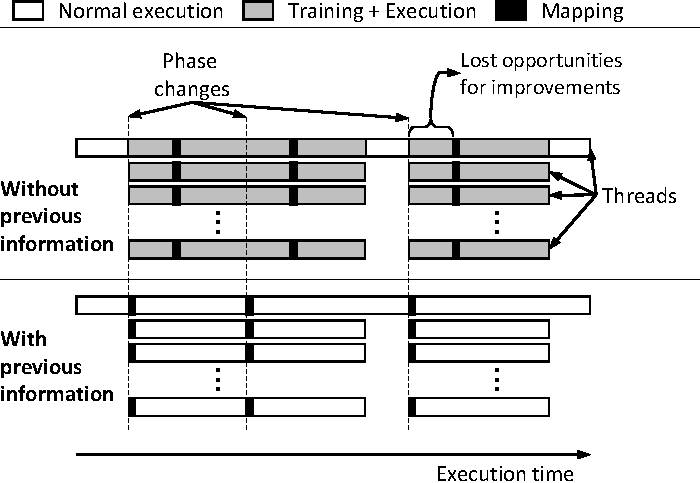
\includegraphics[width=\linewidth]{img/timeline}
%    %!TEX encoding=UTF-8 Unicode
%!TEX root=../tabarnac.tex

\def\len{6}
\def\wid{0.3}
\def\dis{0.1}

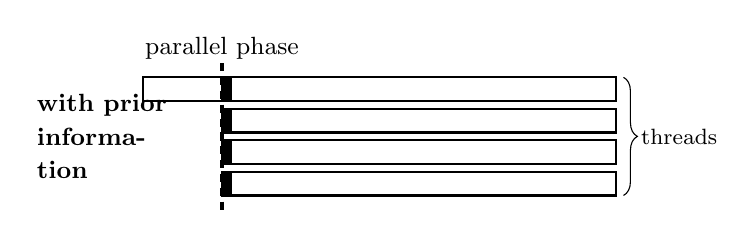
\begin{tikzpicture}
	\node[align=left, text width=1.7cm] at (-0.5,-\wid-1.5*\dis) (label1) {\bfseries\small with prior information};

	\draw[thick] (0,0)              rectangle +(\len, \wid);
	\draw[thick] (1,-\wid*0-\dis*1) rectangle +(\len-1,-\wid);
	\draw[thick] (1,-\wid*1-\dis*2) rectangle +(\len-1,-\wid);
	\draw[thick] (1,-\wid*2-\dis*3) rectangle +(\len-1,-\wid);

	\draw[fill=black] (1,0)              rectangle +(0.12,\wid);
	\draw[fill=black] (1,-\wid*0-\dis*1) rectangle +(0.12,-\wid);
	\draw[fill=black] (1,-\wid*1-\dis*2) rectangle +(0.12,-\wid);
	\draw[fill=black] (1,-\wid*2-\dis*3) rectangle +(0.12,-\wid);

	\draw[very thick,densely dashed] (1,1.6*\wid) -- +(0,-\wid*5-\dis*4.3) node[near start,pos=-0.1] {\small parallel phase};

	\draw [decorate,decoration={brace,amplitude=5pt}] (\len+.1,\wid) -- ++(0,-4*\wid-3*\dis) node [midway,right=1mm]{\footnotesize threads};

	% \draw (-1.35,-\wid*5) -- +(8.8,0); %separator


\end{tikzpicture}


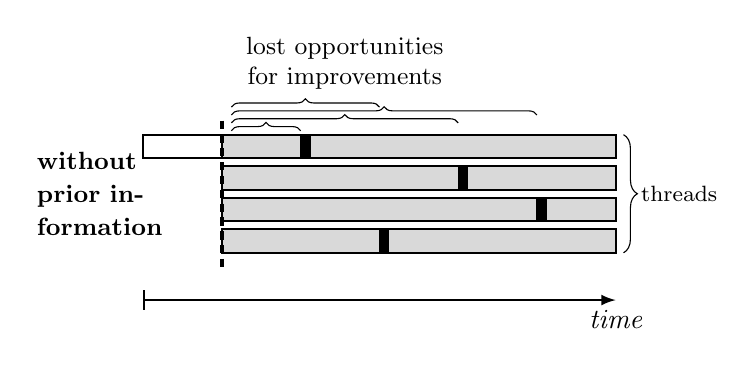
\begin{tikzpicture}
	\node[align=left, text width=2cm] at (-0.35,-\wid-1.5*\dis) (label1) {\bfseries\small without prior information};

	\draw[thick] (0,0)              rectangle +(\len, \wid);
	\draw[fill=gray!30, thick] (1,0)              rectangle +(\len-1, \wid);
	\draw[fill=gray!30, thick] (1,-\wid*0-\dis*1) rectangle +(\len-1,-\wid);
	\draw[fill=gray!30, thick] (1,-\wid*1-\dis*2) rectangle +(\len-1,-\wid);
	\draw[fill=gray!30, thick] (1,-\wid*2-\dis*3) rectangle +(\len-1,-\wid);

	\draw[fill=black] (2,0)              rectangle +(0.12,\wid);
	\draw[fill=black] (4,-\wid*0-\dis*1) rectangle +(0.12,-\wid);
	\draw[fill=black] (5,-\wid*1-\dis*2) rectangle +(0.12,-\wid);
	\draw[fill=black] (3,-\wid*2-\dis*3) rectangle +(0.12,-\wid);

	\draw[decorate,decoration={brace,amplitude=3pt}] (1+0.12,\wid+0.05) -- +(1-0.12,0);
	\draw[decorate,decoration={brace,amplitude=3pt}] (1+0.12,\wid+0.15) -- +(3-0.12,0)node[midway,above=3mm,align=center,font=\small] {\small lost opportunities\\ for improvements};
	\draw[decorate,decoration={brace,amplitude=3pt}] (1+0.12,\wid+0.25) -- +(4-0.12,0);
	\draw[decorate,decoration={brace,amplitude=3pt}] (1+0.12,\wid+0.35) -- +(2-0.12,0);

	\draw[very thick,densely dashed] (1,1.6*\wid) -- +(0,-\wid*5-\dis*4.3);

	\draw[decorate,decoration={brace,amplitude=5pt}] (\len+.1,\wid) -- ++(0,-4*\wid-3*\dis) node [midway,right=1mm]{\footnotesize threads};

	\draw[thick,|-latex] (0,-\wid*6) -- +(\len,0) node[below] {\itshape time};

\end{tikzpicture}

%    \caption{Comparison of data mapping mechanisms with and without prior information about the memory access behavior of a parallel application consisting of four threads. Training is similar to the normal execution, but with additional training overhead.}
%    \label{fig:timeline}
%\end{figure}

\subsubsection{Mechanisms Without Prior Information}
\DB{Can we shorten this part, keep only big ideas ?}
% kernel old
Most mechanisms that have no prior information about the memory access behavior operate within the operating system.
Traditionally, operating systems have used the \emph{first-touch}~\cite{Marchetti1995}, \emph{next-touch}~\cite{Lof2005} and \emph{interleave}~\cite{Kleen2004} policies to map memory pages to NUMA nodes.
The first-touch policy~\cite{Marchetti1995}, which is the default policy in most current operating systems (such as Linux), allocates a page on the NUMA node that performs the first memory access to it.
The page is never migrated between nodes.
First-touch requires that the programmer takes care of which thread accesses data first.
In some circumstances, this policy can lead to reduced performance, for
instance when a single thread initializes a large part of the memory and places most pages on a single node.
In next-touch~\cite{Lof2005}, each page is periodically migrated to the NUMA node that performs the next access to a page.
This policy can lead to excessive page migrations if the memory access behavior is changing fast.
The interleave policy (which is available in Linux via the \texttt{numactl} tool~\cite{Kleen2004} for example) distributes memory pages equally among all NUMA nodes, but does not take any locality of memory accesses into account.

Newer developments in operating systems focus on refining the data mapping during the execution of parallel applications, using online profiling of memory accesses to guide migration decisions.
Recent versions of the Linux kernel (starting with version 3.8) contain the NUMA Balancing technique~\cite{Corbet}, which uses page faults during execution to determine if a page should be migrated to a different NUMA node. To increase the accuracy of this mechanism, extra page faults are inserted during execution, creating an additional overhead.
A similar proposal is the AutoNUMA approach~\cite{Corbet2012}.
Neither mechanism maintains an access history. This eliminates the need to store the access behavior, but also makes them susceptible to excessive migrations.
Other proposals store such an access history.
Dashti et al.~\cite{Dashti2013} introduced the Carrefour mechanism, which uses instruction-based sampling~(IBS)~\cite{Drongowski07Instructionbased} available in recent AMD architectures~\cite{AMD2012} to detect the memory access behavior.
kMAF~\cite{Diener2014} is a similar mechanism that uses page faults to analyze the behavior.
Due to the access history, these mechanisms can avoid excessive migrations, but still suffer from later migrations and a runtime overhead compared to mechanisms with prior information.

% hardware
% marathe, lapt

\subsubsection{Mechanisms With Prior Information}

Most mechanisms with prior information about memory access behavior perform mapping in user space, on the compiler or runtime library level.
Piccoli et al.~\cite{Piccoli2014} propose a compiler extension that analyzes the memory access pattern of loops that are executed in parallel and use this information to migrate pages before the loop is entered.
Nikolopoulos et al.~\cite{Nikolopoulos2000a,Nikolopoulos2000} present an integrated compiler/OS-based data mapping mechanism based on a custom OpenMP compiler and IRIX kernel extensions. The compiler inserts instrumentation code to identify access patterns to shared memory areas and to guide migration decisions.
ForestGOMP~\cite{Broquedis2010a} requires source code annotations to identify memory access behavior and is limited to the OpenMP library.
These techniques use predictions about the memory access behavior, which might be dependent on input data and can cause wrong mappings.
Furthermore, no improvements to the memory access pattern are performed.

Libraries that support NUMA-aware memory allocation include libnuma~\cite{Kleen2004} and MAi~\cite{Ribeiro2009}. With these libraries, data structures can be allocated according to the specification of the programmer, such as on a particular NUMA node, or with an interleave policy. These techniques can achieve large improvements, but place the burden of the mapping on the programmer, who has to determine the best placement himself.
% An evolution of MAi, the Minas framework~\cite{Ribeiro2010}, optionally uses a source code preprocessor to determine data mapping policies for arrays.
%
Previous research also uses memory access traces to perform data mapping~\cite{Diener2015,Marathe2010,Bolosky1992}. These can be useful to determine the maximum gains that can be achieved with mapping policies, but are not applicable in general due to their substantial overhead and the fact that the access behavior might change with different input data and different numbers of threads, for instance.
Generic tools to evaluate parallel application performance, such as Intel's VTune~\cite{Reinders05VTune} and Performance Counter Monitor~(PCM)~\cite{Intel2012b}, the HPCToolkit~\cite{Adhianto10HPCTOOLKIT}, and AMD's CodeAnalyst~\cite{Drongowski2008}, provide only indirect information about the memory access behavior and do not propose specific strategies to improve it.


\subsection{Memory Profiling}
\label{sec:soa-profiling}

Profiling memory behavior raise two main challenges, first collecting the
information: if performance counters have been developed to get quick and
easy access to information about the CPU usage, there is no such mechanism for
the memory. Second memory access traces provides huge amounts of information
on several dimension (data structure, threads, access type (read/write),
sharing, time \ldots) displaying them to the user in a readable and meaningful
way is therefore not trivial.

\subsubsection{Data collection}

Several methods have been used to address the problem of data collection. A
lot of studies tries to deduce information from hardware performance
counters~\cite{Majo13(Mis)understanding,
Jiang14Understanding,Bosch00Rivet,Weyers14Visualization,Tao01Visualizing,DeRose01Hardware},
the special register allows to record events such as cache misses and remote
memory accesses, among others. Still, these counters only provide a partial
view of the execution, they show events happening on the processor related to
memory, but not what triggered them. Moreover available performance counters
depends of the architecture therefore it is hard to reproduce the same
analysis on different machines with these tools.


Another approach used by several
tools~\cite{Lachaize12MemProf,McCurdy2010,Liu14Tool,Gimenez14Dissecting}
consist on  using sampling mechanisms such as AMD's Instruction Based Sampling
(IBS) or Intel PEBS. Not only can sampling miss important events, leading to
inaccurate characterizations, but these technologies are not portable and work
only with a few recent architecture, therefore such tools can only be used in
special circumstances.

Other studies uses hardware modification (with or without simulator)
\cite{Bao08HMTT,Martonosi92MemSpy}, although it provides efficient trace
collection it is even less portable.


Finally, instrumentation can provide these informations as in
\cite{DeRose02SIGMA,Rozar14Amelioration}, although this method is slower than
the other previously described, it is more portable and precise. Moreover as
we show in section \ref{sec:expe-overhead} an efficient instrumentation
provides an acceptable overhead.

\subsubsection{Visualization}

The second difficulty of memory analysis is to present the information in such
a way that the user can use it to improve the application. Some of the tools
previously mentioned only provide a textual
output~\cite{Lachaize12MemProf,McCurdy2010,Martonosi92MemSpy}. Even if these
tools highlight the most relevant informations, it is hard to get an overview
of the memory behavior from such output. The user might be faced with a huge
amount of information and not be able to differentiate normal behaviors from
problematic ones.


Other tools provide more advanced visualizations. For
instance, Tao et al.~\cite{Tao01Visualizing} propose a detailed view of each memory
page, showing the number of remote and local accesses from each NUMA node. Weyers et
al.~\cite{Weyers14Visualization} depict the memory bandwidth between each pair of nodes,
showing where the remote accesses occur. Other
tools~\cite{DeRose01Hardware,DeRose02SIGMA,Bosch00Rivet} provide several views
of the execution, giving the ability to correlate them with the source code as
we are used to do with traditional performance tools such as Vtune.

Although all these tools can help developers and users to understand the kind of performance issues they are facing, they never give the
reason \emph{why} the issue is happening, or how to improve it.

Gimenez et al.~\cite{Gimenez14Dissecting} provides a NUMA oriented view of the
execution, showing which node is responsible of how many access, moreover they
provides \emph{parallel coordinate graphs} to understand where does memory
problems comes from. Still it requires a lot of experiment to the user to
understand these graphs.

Finally Liu et al.'s work~\cite{Liu14Tool} is quite near to the previous studies but
they also show some \emph{address centric} visualization which helps answering
why the performance issue occurred. However these views are not enough mature
yet and only answer a part of the question.

%Previous studies aimed to answer this question for some specific
%benchmarks~\cite{Majo13(Mis)understanding,Jiang14Understanding}.
%However, these studies use manual source code analysis and performance counters and do not provide a general tool or methodology that is usable for other applications.

\subsection{Summary of Related Work}

Summarizing our discussion of previous work in this area, we conclude that tools to improve the memory access behavior on NUMA architectures with prior information have the highest potential for improvements.
The two main challenges for this type of tool is to gather information about the memory access patterns in a fast, accurate and easy-to-use way, and providing information to the developers about the ways to improve the behavior of their applications.
This study, provides a comprehensive solution for these challenges.

% \MD{mechanisms with prior information have highest potential for improvements, but currently:
% - lack of information about memory access behavior
% - lack of information about ways to improve behavior
% }
% Importance of Mapping:
% \begin{itemize}
%     \item First touch
%     \item Interleave
% \end{itemize}

% Why Not automated tools
% \begin{itemize}
%     \item Trainning time
%     \item Garbage in/ garbage out (matrix modulo / bloc)
% \end{itemize}

% New tool: understand why performances are bad
